% !TEX encoding = UTF-8 Unicode.

% Based on https://github.com/Miracle0565/BUCT-Beamer-Theme

\documentclass[
10pt,
aspectratio=43,
]{beamer}
\setbeamercovered{transparent=10}
\usetheme[
%  showheader,
%  red,
  purple,
%  gray,
%  graytitle,
  colorblocks,
%  noframetitlerule,
]{Verona}

\usepackage[T1]{fontenc}
\usepackage{tikz}
\usepackage[utf8]{inputenc}
\usepackage{lipsum}
%%%%%%%%%%%%%%%%%%%%%%%%%%%%%%%
% Mac上使用如下命令声明隶书字体, windows也有相关方式, 大家可自行修改
\providecommand{\lishu}{\CJKfamily{zhli}}
%%%%%%%%%%%%%%%%%%%%%%%%%%%%%%%
\usepackage{tikz}
\usetikzlibrary{fadings}
%
%\setbeamertemplate{sections/subsections in toc}[ball]
\usepackage{xeCJK}
\usepackage{listings}
\usepackage{caption}
\usepackage{subfigure}
\usefonttheme{professionalfonts}
\def\mathfamilydefault{\rmdefault}
\usepackage{amsmath}
\usepackage{multirow}
\usepackage{booktabs}
\usepackage{bm}
\usepackage{mathtools}
\usepackage[T1]{fontenc}
\setbeamertemplate{section in toc}{\hspace*{1em}\inserttocsectionnumber.~\inserttocsection\par}
\setbeamertemplate{subsection in toc}{\hspace*{2em}\inserttocsectionnumber.\inserttocsubsectionnumber.~\inserttocsubsection\par}
\setbeamerfont{subsection in toc}{size=\small}
\AtBeginSection[]{%
	\begin{frame}%
		\frametitle{Outline}%
		\textbf{\tableofcontents[currentsection]} %
	\end{frame}%
}

\AtBeginSubsection[]{%
	\begin{frame}%
		\frametitle{Outline}%
		\textbf{\tableofcontents[currentsection, currentsubsection]} %
	\end{frame}%
}

\title{高等数学C}
%\subtitle{A Simple while elegant template}
\author[P.Yu]{余沛}
\mail{peiy\_gzgs@qq.com}
\institute[Guangzhou College of Technology and Business]{Guangzhou College of Technology and Business \\
  广州工商学院}
\date{\today}
\titlegraphic[width=4cm]{logo.png}{}




%%%%%%%%%%%%%%%%%%%%%%%%%%%%%%%%
% ----------- 标题页 ------------
%%%%%%%%%%%%%%%%%%%%%%%%%%%%%%%%



\begin{document}

\maketitle

%%% define code
\defverbatim[colored]\lstI{
	\begin{lstlisting}[language=C++,basicstyle=\ttfamily,keywordstyle=\color{red}]
	int main() {
	// Define variables at the beginning
	// of the block, as in C:
	CStash intStash, stringStash;
	int i;
	char* cp;
	ifstream in;
	string line;
	[...]
	\end{lstlisting}
}
%%%%%%%%%%%%%%%%%%%%%%%%%%%%%%%%
% ----------- FRAME ------------
%%%%%%%%%%%%%%%%%%%%%%%%%%%%%%%%

\section{不定积分的概念}

\subsection{算子, 逆算子, 微分算子, 微分逆算子, 原函数, 不定积分}
\begin{frame}
	\frametitle{算子和逆算子}
	{\small
		\begin{block}{算子}
			算子是指将集合中的元素指向另一个元素的映射. 在这里我们先用大写字母表示, 比如$A$和$B$.
		\end{block}
		\pause
		\begin{block}{逆算子}
			给定一个算子$A$, 如果存在另一个算子$B$, 使得$A$和$B$的复合运算等于单位算子$I$(恒等映射), 即$AB=BA=I$, 则称$B$是$A$的逆算子, 记作 $B=A^{-1}$.
		\end{block}
		\pause
		\begin{exampleblock}{例子:数乘算子与数乘算子的逆}
			考虑数乘算子$A$, 它将实数$x$映射到它的2倍, 即$A(x) = 2x$. 那么$A$的逆算子$B$将实数$x$映射到一半, 即$B(x) = \frac{1}{2}x$. 在这个例子中, $B$是数除算子. \pause $B=A^{-1}$, 这个求逆运算也是减法计算的来源.
		\end{exampleblock}
		\pause
		\begin{exampleblock}{例子:数加算子与数加算子的逆}
			考虑数加算子$A$, 它将实数$x$映射到它加$1$, 即$A(x) = x+1$. 那么$A$的逆算子$B$将实数$x$映射到它减一, 即$B(x) = x-1$. 在这个例子中, $B$就是数减算子. \pause $B=A^{-1}$, 这个求逆运算也是除法计算的来源.
		\end{exampleblock}
	}
\end{frame}

\begin{frame}
	\frametitle{微分算子}
	回顾到微分运算, 回顾微分运算的本质:
	\begin{block}{微分算子}
		在微积分中, 微分算子是指将一个函数映射到它的导数的操作符.
		$$
			\frac{\mathrm{~d}}{\mathrm{~d}x}f(x)=f'(x)
		$$
		在这里, 我们用标准的微分符号$\frac{\mathrm{~d}}{\mathrm{~d}x}$来描述某个自变量为 $x$ 的函数的微分算子.
	\end{block}
	\pause
	\vspace{0.2cm}
	\vfill
	\centering
	{
		\centering
		那么
	}
	\pause
	\vfill
	\centering
	{
		\centering
		微分算子的逆运算是什么? \pause 姑且先记录为 $\displaystyle\left(\frac{\mathrm{~d}}{\mathrm{~d}x}\right)^{-1}$. \pause 又会有什么作用?
	}
\end{frame}

\begin{frame}
	\frametitle{微分算子的逆}
	\begin{block}{}
		要对算子 $\left(\frac{\mathrm{~d}}{\mathrm{~d}x}\right)^{-1}$ 进行刻画, \pause 就要问以下两个问题:
		\vspace{0.3cm}
		\begin{enumerate}
			\pause
			\item 对于哪些函数来说, 有
			      $$
				      \displaystyle\left(\frac{\mathrm{~d}}{\mathrm{~d}x}\right)^{-1}\left(\frac{\mathrm{~d}}{\mathrm{~d}x}\right)=I?
			      $$
			      \vspace{0.2cm}
			      \pause
			\item $\displaystyle\left(\frac{\mathrm{~d}}{\mathrm{~d}x}\right)^{-1}$ 应当怎么计算?
		\end{enumerate}
		\vspace{0.3cm}
	\end{block}
\end{frame}

\begin{frame}
	\frametitle{逆算子: 原函数与原函数的唯一性}
	首先我们给出原函数的概念:
	\begin{block}{}
		对于函数$f(x)$, 如果存在函数 $F(x)$ 满足 $\frac{\mathrm{~d}}{\mathrm{~d}x} F(x) = f(x)$, 那么自然地,
		$$
			F(x)=\displaystyle\left(\frac{\mathrm{~d}}{\mathrm{~d}x}\right)^{-1}f(x).
		$$
		在这种情况下, 我们称 $F(x)$ 为 $f(x)$ 的原函数.
	\end{block}
	\pause
	我们可以看到, 原函数是不唯一的.
	\pause
	\begin{block}{}
		对于函数$f(x)$, 假如 $F(x)$ 为 $f(x)$ 的原函数, 那么对于任意常数 $C$, 可以发现 $\frac{\mathrm{~d}}{\mathrm{~d}x} \left(F(x)+C\right) = f(x)$ 也成立.
	\end{block}
	\pause
	\begin{block}{}
		\vfill
		\centering
		{
			\centering
			没想到吧!
		}
	\end{block}
	但是但是, 如果我们不考虑这个常数, 那么连续函数的原函数其实是唯一的.
\end{frame}

\begin{frame}
	\frametitle{逆算子: 原函数与原函数的唯一性}
	\begin{theorem}
		连续函数 $f(x)$ 存在原函数, 而且对于任意两个原函数 $F_1(x)$ 和 $F_2(x)$ 只差一个常数, 即 存在常数 $C$ 使得 $F(x)-G(x)=C$.
	\end{theorem}
	\begin{block}{Proof.}
		我们先证明唯一性, 可以发现
		$$
			(F(x)-G(x))'=f(x)-f(x)=0.
		$$
		由于Lagrange中值定理, 假如 $F(x)-G(x)\neq C$, 对于任意 不满足 $(F(x_1)-G(x_1))-(F(x_2)-G(x_2))=0$ 的 $x_1, x_2$, 存在 $\xi\in(x_1,x_2)$, 满足
		$$
			(F(\xi)-G(\xi))'=\frac{(F(x_1)-G(x_1))-(F(x_2)-G(x_2))}{x_1-x_2}\neq 0.
		$$
		存在性将在学习定积分的时候给出, 有一个具体的计算方法.
		\qed
	\end{block}
\end{frame}

\begin{frame}
	\frametitle{微分算子的逆: 不定积分算子}

	微分算子的逆, \pause 这种函数$f(x)$到原函数$F(x)$的算子一般被称为:
	$$
		\text{不定积分算子:}\pause\,\,\,\, \int\cdot\,\,\mathrm{~d}x:\,\,\pause f(x)\rightarrow F(x)\pause +C.
	$$

	\pause 这里的 $+C$ 是为了说明差一个常数, \pause $\int\cdot\,\,\mathrm{~d}x$ 是所谓的 Leibniz 记号.
	\vspace{0.2cm}

	这记号的好处是, 对于微分计算$f(x)\mathrm{~d}x=\mathrm{~d}F(x)$
	\vspace{0.2cm}
	$$
		\int f(x) \mathrm{~d}x = \int \mathrm{~d} F(x) = F(x) +C,\quad \text{及}\quad \mathrm{~d}\left(\int f(x)\mathrm{~d}x\right) = f(x).
	$$
	\vspace{0.2cm}
	\pause 该记号能够更好地将微分算子 $\mathrm{~d}$ 和 积分算子 $\int $(微分算子的逆算) 具有 $\mathrm{~d}\int=\int \mathrm{~d}= I $(相差一个常数)的性质.
\end{frame}

\begin{frame}
	\frametitle{来点练习}
	\everymath{\displaystyle}
	最最标准的求不定积分的方法是直接找到对应的原函数.
	{\small
	\pause
	\begin{exampleblock}{证明: $\color{black}\int x^5 \mathrm{~d} x=\frac{1}{6} x^6+C$}
		\pause
		$
			\left(\frac{1}{6} x^6\right)^{\prime}=x^5 \pause \Rightarrow \int x^5 d x=\frac{1}{6} x^6+C.
		$
	\end{exampleblock}
	\pause
	\begin{exampleblock}{证明: $\color{black}\int \frac1x \mathrm{~d} x=\ln |x|+C$}
		\pause
		对于 $x>0$ 的情况, 有
		$
			(\ln x)^{\prime}=\frac{1}{x} \Rightarrow \int \frac{1}{x} \mathrm{~d} x=\ln x+C.
		$
		\pause

		对于 $x<0$ 的情况, 有
		$
			(\ln (-x))'=\frac{1}{-x}(-x)^{\prime}=\frac{1}{x} \Rightarrow \int \frac{1}{x} \mathrm{~d} x=\ln -x+C.
		$
	\end{exampleblock}
	\pause
	\begin{exampleblock}{证明: $\color{black}\int \frac{\mathrm{~d} x}{\cos ^2 x}=\tan x+C$}
		\pause
		$
			\int \frac{\mathrm{~d} x}{\cos ^2 x}=\pause\int \sec ^2 x \mathrm{~d} x=\pause\int \mathrm{~d} \tan x=\pause\tan x+ C.
		$
	\end{exampleblock}
	}
\end{frame}

\subsection{基本不定积分公式和基本微分公式}
\begin{frame}
	\frametitle{从微分公式到积分公式}
	\everymath{\displaystyle}
	\renewcommand{\arraystretch}{2.3}
	\resizebox{\linewidth}{!}
	{
		\begin{tabular}{|p{0.35\textwidth}|p{0.45\textwidth}|}
			\hline
			$\mathrm{~d}x^a=ax^{a-1}\mathrm{~d}x$, $a\neq0$                   & $\int x^{a-1}\mathrm{~d}x=\frac{1}{a}x^{a}+C$, $a\neq0$  \\
			\hline
			$\mathrm{~d}\sin x=\cos x\mathrm{~d}x$                            & $\int \cos x\mathrm{~d}x = \sin x+C$                     \\
			\hline
			$\mathrm{~d}\cos x=-\sin x\mathrm{~d}x$                           & $\int \sin x\mathrm{~d}x=-\cos x +C$                     \\
			\hline
			$\mathrm{~d}\log_ax=\frac{1}{\log a}\cdot\frac{1}{x}\mathrm{~d}x$ & $\int \frac{1}{x}\mathrm{~d}x = \log |x|+C$              \\
			\hline
			$\mathrm{~d}a^x=\log a^x\mathrm{~d}x$                             & $\int a^x\mathrm{~d}x = \frac{1}{\log a}a^x+C$           \\
			\hline
			$\mathrm{~d}\arcsin x =\frac{1}{\sqrt{1-x^2}}\mathrm{~d}x$        & $\int \frac{1}{\sqrt{1-x^2}}\mathrm{~d}x = \arcsin x +C$ \\
			\hline
			$\mathrm{~d}\arctan x =\frac{1}{1+x^2}\mathrm{~d}x$               & $\int \frac{1}{1+x^2}\mathrm{~d}x = \arctan x +C$        \\
			\hline
		\end{tabular}
	}
\end{frame}



\begin{frame}
	\frametitle{从微分计算法则到不定积分计算法则}
	接下来我们回顾微分计算法则, 并导出重要的不定积分计算法则:\pause
	\begin{block}{}
		\begin{enumerate}
			\item 线性叠加法则:
			      \begin{itemize}
				      \item \pause 假设$k, l$为实数, $u, v$ 为函数微分的和差法则和数乘法则:
				            $$
					            (ku'+lv')\mathrm{~d}x=\mathrm{~d}(ku+ lv) = \mathrm{~d}ku + \mathrm{~d}lv=ku'\mathrm{~d}x+lv'\mathrm{~d}x.
				            $$
				      \item \pause 不定积分的和差法则:
				            $$
					            \int(ku'+lv')\mathrm{d}x=\int\mathrm{d}(ku+ lv) = \int k\mathrm{d}u + l\mathrm{d}v=k\int u'\mathrm{~d}x+l\int v'\mathrm{~d}x.
				            $$
			      \end{itemize}
			      \pause
			\item 乘积法则:
			      \begin{itemize}
				      \item \pause 微分的乘积法则:
				            $$
					            u\mathrm{~d}v+v\mathrm{~d}u =\mathrm{~d}(uv).
				            $$
				      \item \pause 不定积分的乘积法则:
				            $$
					            \int u\mathrm{~d}v+\int v\mathrm{~d}u=\int\mathrm{~d}(uv) = uv.
				            $$
				            \pause 最后这一条经常被称为分部积分公式.
			      \end{itemize}
		\end{enumerate}
	\end{block}
\end{frame}

\begin{frame}
	\frametitle{从微分计算法则到不定积分计算法则}
	\begin{block}{}
		\begin{enumerate}\setcounter{enumi}{2}
			 \item 商法则:
			      \begin{itemize}
				       \item 微分的商法则
				            $$
					            \mathrm{~d}\left(\frac{u}{v}\right)=\frac{u\mathrm{~d}v-v\mathrm{~d}u}{v^2}.
				            $$
				             \item 不定积分的商法则  (基本不会用到这个法则)
				            $$
					            \frac{u}{v}=\int \frac{u}{v^2}\mathrm{~d}v-\int\frac{1}{v}\mathrm{~d}u.
				            $$

			      \end{itemize}
			       \item 复合函数微分法则:
			      \begin{itemize}
				      \item 微分的复合函数求导法则, 设$f(x)$ 和 $g(x)$ 是可导函数,记 $h(x) = f(g(x))$
				            $$
					            f'(g(x))g'(x)\mathrm{~d}x=f'(g(x))\mathrm{~d}g(x)=\mathrm{~d}h(x).
				            $$
				      \item  不定积分的和差法则
				            $$
					            \int f'(g(x))g'(x)\mathrm{~d}x=\int f'(g(x))\mathrm{~d}g(x)=\int \mathrm{~d}h(x)= h(x)+C.
				            $$
			      \end{itemize}
		\end{enumerate}
	\end{block}
\end{frame}

\subsection{熟悉直接积分法}
\begin{frame}
	\frametitle{熟悉直接积分法}
	\everymath{\displaystyle}
	{\small
		\begin{exampleblock}{$\color{black}\int \sqrt{x}\left(x^2-5\right) \mathrm{~d} x$}
			$
				\int \sqrt{x}\left(x^2-5\right) \mathrm{~d}x= \pause \int x^{\frac{5}{2}}\mathrm{~d}x-\int 5x^{\frac{1}{2}} \mathrm{~d}x \pause =\frac{7}{2}x^{\frac{7}{2}}-\frac{10}{3}x^{\frac{3}{2}}+C.
			$
		\end{exampleblock}
		\pause
		\begin{exampleblock}{$\color{black}\int \frac{(x-1)^3}{x^2} \mathrm{~d} x$}
			$
				\int \frac{(x-1)^3}{x^2} \mathrm{~d} x= \pause \int x-3+3\frac{1}{x}-\frac{1}{x^2} \mathrm{~d}x= \pause \frac{1}{2}x^2-3x+3\log|x|+\frac{1}{x}+C.
			$
		\end{exampleblock}
		\pause
		\begin{exampleblock}{$\color{black}\int\left(e^x-3 \cos x\right) \mathrm{~d} x$}
			$
				\int\left(e^x-3 \cos x\right) \mathrm{~d} x=\pause\int e^x\mathrm{~d} x-3 \int\cos x \mathrm{~d} x=\pause e^x-3\sin x+C.
			$
		\end{exampleblock}
	}
\end{frame}

\begin{frame}
	\frametitle{熟悉直接积分法}
	\everymath{\displaystyle}
	{\small
		\begin{exampleblock}{$\color{black}\int \frac{2 x^4+x^2+3}{x^2+1} \mathrm{~d} x$}
			$
				\int \frac{2 x^4+x^2+3}{x^2+1} \mathrm{~d} x =\pause \int \frac{2 x^4+2x^2}{x^2+1}+\frac{-x^2+3}{x^2+1} \mathrm{~d} x =\pause \int 2x^2-1+4 \frac{1}{x^2+1}\mathrm{~d} x,
			$
			\pause
			$
				\int \frac{2 x^4+x^2+3}{x^2+1} \mathrm{~d} x = \pause\frac{2}{3}x^3-x+4\arctan x+ C.
			$
		\end{exampleblock}
		\pause
		\begin{exampleblock}{$\color{black}\int \tan^2 x \mathrm{~d} x$}
			$
				\int \tan^2 x \mathrm{~d} x =\pause \int \frac{\sin^2 x}{\cos^2}\mathrm{~d} x =\pause \int \frac{1}{\cos^2 x}-1\mathrm{~d} x=\tan x-x+C.
			$
		\end{exampleblock}
		\pause
		\begin{exampleblock}{$\color{black}\int \frac{1}{\sin ^2 \frac{x}{2} \cos ^2 \frac{x}{2}} \mathrm{~d} x$}
			$
				\int \frac{1}{\sin ^2 \frac{x}{2} \cos ^2 \frac{x}{2}} \mathrm{~d} x =\pause \int \frac{1}{(\frac{1}{2}\sin x)^2} \mathrm{~d} x =\pause \int \frac{4}{\sin^2 x}\mathrm{~d} x=\pause-4\cot x+C.
			$
		\end{exampleblock}
	}
\end{frame}

\begin{frame}
	\frametitle{熟悉直接积分法}
	\everymath{\displaystyle}
	{\small
		\begin{exampleblock}{$\color{black}\int \frac{\mathrm{~d} x}{1-x^2}$}
			$
				\int \frac{\mathrm{~d} x}{1-x^2}= \int \frac{1}{(1-x)(1+x)}\mathrm{~d} x=\frac{1}{2}\int \left(\frac{1}{1-x}+\frac{1}{1+x}\right)\mathrm{~d} x,
			$
			\\
			$
				\int \frac{\mathrm{~d} x}{1-x^2}=\frac{1}{2}(\log|1+x|-\log|1-x|)+C=\frac{1}{2}\log\left|\frac{1+x}{1-x}\right|+C.
			$
		\end{exampleblock}
		\pause
		\begin{alertblock}{$\color{black}\int \frac{\mathrm{~d} x}{\sqrt{x^2 \pm 1}}$}
			$
				x>0\,\,\text{case:}\,\, \left(\ln|x+\sqrt{x^2\pm1}|\right)'=\frac{1}{x+\sqrt{x^2\pm1}}\cdot\left(1+\frac{x}{\sqrt{x^2\pm1}}\right)=\frac{1}{\sqrt{x^2\pm1}}.
			$
			\\\vspace{0.2cm}
			$
				x<0\,\,\text{case:}\,\, \left(\ln(-x+\sqrt{x^2-1})\right)'=\frac{1}{-x+\sqrt{x^2-1}}\cdot\left(-1+\frac{x}{\sqrt{x^2-1}}\right)=\frac{1}{\sqrt{x^2-1}}.
			$
		\end{alertblock}
	}
\end{frame}

\section{基本积分法}

\subsection{变量代换方法一: 凑微分法}


\begin{frame}
	\frametitle{凑微分法}
	\everymath{\displaystyle}
	回顾不定积分的复合运算法则
	$$
		\int f'(g(x))g'(x)\mathrm{~d}x=\int f'(g(x))\mathrm{~d}g(x)=\int \mathrm{~d}f(g(x))= f(g(x))+C.
	$$
	\pause
	用这种办法, 如果能用函数凑出因子 $g'(x)$, 而 $g(x)$ 作为变量时, 能简化计算...这种方法就称为凑微分法.
	\vspace{0.3cm}

	来看一个例子:
	\pause
	\vspace{0.1cm}
	\begin{exampleblock}{$\color{black}\int(2 x+1)^6 \mathrm{~d} x$}
		$$
			\begin{aligned}
				\int(2 x+1)^6 \mathrm{~d} x & \pause=  \int(2 x+1)^6 \frac{1}{2}\cdot 2 \mathrm{~d} x \\
				                            & \pause=  \frac{1}{2}\int(2 x+1)^6 \mathrm{~d} (2x+1)    \\
				                            & \pause= \frac{1}{14}(2x+1)^7+C.
			\end{aligned}
		$$
	\end{exampleblock}

\end{frame}

\begin{frame}
	\frametitle{凑微分法}
	\everymath{\displaystyle}
	\begin{exampleblock}{$\color{black}\int x \sqrt{1-x^2} \mathrm{~d} x$}
		$$
			\begin{aligned}
				\int x \sqrt{1-x^2} \mathrm{~d} x & \pause= -\frac{1}{2} \int \sqrt{1-x^2} \mathrm{~d}\left(1-x^2\right)      \\
				                                  & \pause= -\frac{1}{2} \cdot \frac{2}{3}\left(1-x^2\right)^{\frac{3}{2}}+C.
			\end{aligned}
		$$
	\end{exampleblock}
	\pause
	\begin{exampleblock}{$\color{black}\int (3x+2)^{100} \mathrm{~d}x$}
		$$
			\begin{aligned}
				\int (3x+2)^{100} \mathrm{~d}x      & \pause= \frac{1}{3} \int (3x+2)^{100} \mathrm{~d}(3x+2)               \\
				\pause\underline{\text{let }u=3x+2} & \pause=  \frac{1}{3} \int u^{100} \mathrm{~d}u                        \\
				                                    & \pause= \frac{1}{303} u^{101}+C \pause = \frac{1}{303}(3x+2)^{101}+C.
			\end{aligned}
		$$
	\end{exampleblock}
\end{frame}

\begin{frame}
	\frametitle{凑微分法}
	\everymath{\displaystyle}
	{\small
		\begin{exampleblock}{$\color{black}\int x e^{x^2} \mathrm{~d}x$}
			$$
				\begin{aligned}
					\int x e^{x^2} \mathrm{~d}x        & \pause= \frac{1}{2} \int e^{x^2} \mathrm{~d}(x^2)        \\
					\pause\underline{\text{let }u=x^2} & \pause=  \frac{1}{2} \int e^u \mathrm{~d}u               \\
					                                   & \pause= \frac{1}{2} e^u+C \pause= \frac{1}{2} e^{x^2}+C.
				\end{aligned}
			$$
		\end{exampleblock}
		\pause
		\begin{exampleblock}{$\color{black}\int x^4 \cos x^5 \mathrm{~d}x$}
			$$
				\begin{aligned}
					\int x^4 \cos x^5 \mathrm{~d}x     & \pause = \frac{1}{5} \int \cos x^5 \mathrm{~d}(x^5)           \\
					\pause\underline{\text{let }u=x^5} & \pause =  \frac{1}{5} \int \cos u \mathrm{~d}u                \\
					                                   & \pause = \frac{1}{5} \sin u+C =\pause \frac{1}{5} \sin x^5+C.
				\end{aligned}
			$$
		\end{exampleblock}
	}
\end{frame}


\begin{frame}
	\frametitle{凑微分法}
	\everymath{\displaystyle}
	{\small
		\begin{exampleblock}{$\color{black}\int \frac{x}{\sqrt{1-x^4}} \mathrm{~d}x$}
			$$
				\begin{aligned}
					\int \frac{x}{\sqrt{1-x^4}} \mathrm{~d}x & \pause= \frac{1}{2} \int \frac{\mathrm{~d}(x^2)}{\sqrt{1-x^4}}     \\
					\pause\underline{\text{let }u=x^2}       & \pause=  \frac{1}{2} \int \frac{\mathrm{~d}u}{\sqrt{1-u^2}}        \\
					                                         & \pause= \frac{1}{2} \arcsin u+C \pause= \frac{1}{2} \arcsin x^2+C.
				\end{aligned}
			$$
		\end{exampleblock}
		\pause
		\begin{exampleblock}{$\color{black}\int \frac{\mathrm{~d}x}{x(1+2 \ln x)}$}
			$$
				\begin{aligned}
					\int \frac{\mathrm{~d}x}{x(1+2 \ln x)}   & \pause= \int \frac{1}{1+2 \ln x} \mathrm{~d}(\ln x)                  \\
					\pause\underline{\text{let }u=1+2 \ln x} & \pause=  \frac{1}{2} \int \frac{1}{1+2 \ln x} \mathrm{~d}(1+2 \ln x) \\
					                                         & \pause= \frac{1}{2} \ln |1+2 \ln x|+C.
				\end{aligned}
			$$
		\end{exampleblock}
	}
\end{frame}


\begin{frame}
	\frametitle{凑微分法}
	\everymath{\displaystyle}
	{\small
		\begin{exampleblock}{$\color{black}\int \frac{1}{a^2+x^2} \mathrm{~d}x\,\,(a>0)$}
			$$
				\begin{aligned}
					\int \frac{1}{a^2+x^2} \mathrm{~d}x        & \pause = \frac{1}{a^2} \int \frac{1}{1+\frac{x^2}{a^2}} \mathrm{~d}x                     \\
					\pause\underline{\text{let }u=\frac{x}{a}} & \pause =  \frac{1}{a} \int \frac{1}{1+u^2} \mathrm{~d}u                                  \\
					                                           & \pause = \frac{1}{a} \arctan u+C \pause = \frac{1}{a} \arctan\left(\frac{x}{a}\right)+C.
				\end{aligned}
			$$
		\end{exampleblock}
		\pause
		\begin{exampleblock}{$\color{black}\int \frac{1}{\sqrt{a^2-x^2}} \mathrm{~d}x$}
			$$
				\begin{aligned}
					\int \frac{1}{\sqrt{a^2-x^2}} \mathrm{~d}x & \pause = \frac{1}{a} \int \frac{a}{\sqrt{1-\left(\frac{x}{a}\right)^2}} \mathrm{~d}\left(\frac{x}{a}\right) \\
					\pause\underline{\text{let }u=\frac{x}{a}} & \pause =  \frac{1}{a} \int \frac{1}{\sqrt{1-u^2}} \mathrm{~d}u                                              \\
					                                           & \pause = \arcsin(u)+C \pause = \arcsin\left(\frac{x}{a}\right)+C.
				\end{aligned}
			$$
		\end{exampleblock}
	}
\end{frame}


\begin{frame}
	\frametitle{凑微分法}
	\everymath{\displaystyle}
	\begin{exampleblock}{$\color{black}\int \frac{1}{x^2-a^2} \mathrm{~d}x$}
		$$
			\begin{aligned}
				\int \frac{1}{x^2-a^2} \mathrm{~d}x & \pause  = \frac{1}{2a} \int \left(\frac{1}{x-a}-\frac{1}{x+a}\right) \mathrm{~d}x \\
				                                    & \pause = \frac{1}{2a}(\ln |x-a|-\ln |x+a|)+C                                      \\
				                                    & \pause  = \frac{1}{2a} \ln \left|\frac{x-a}{x+a}\right|+C.
			\end{aligned}
		$$
	\end{exampleblock}
	\pause
	\begin{exampleblock}{$\color{black}\int \csc x \mathrm{~d}x$}
		$
			\int \sec x \mathrm{~d}x   = \int \csc x \mathrm{~d} x=\int \frac{\mathrm{d} x}{\sin x}=\int \frac{\mathrm{d} x}{2 \sin \frac{x}{2} \cos \frac{x}{2}}=\int \frac{\mathrm{d}\left(\frac{x}{2}\right)}{\tan \frac{x}{2} \cos ^2 \frac{x}{2}},
		$\\
		$
			\int \sec x \mathrm{~d}x =\ln \left|\tan \frac{x}{2}\right|+C  =\ln |\csc x-\cot x|+C
		$
	\end{exampleblock}
\end{frame}

\begin{frame}
	\frametitle{凑微分法}
	\everymath{\displaystyle}
	\begin{block}{}
		\begin{columns}[onlytextwidth]
			\begin{column}{0.5\textwidth}
				\begin{enumerate}
					\item $\int \frac{\mathrm{~d} x}{x(1+2 \ln x)}$
					\item $\int \frac{e^{3 \sqrt{x}}}{\sqrt{x}} \mathrm{~d} x$
					\item $\int \sec ^6 x d x$
				\end{enumerate}
			\end{column}
			\begin{column}{0.5\textwidth}
				\begin{enumerate}
					\setcounter{enumi}{3}
					\item $\int \sin ^3 x \mathrm{~d} x$
					\item $\int \sin ^2 x \cos ^5 x \mathrm{~d} x$
					\item $\int \tan ^5 x \sec ^3 x d x$
				\end{enumerate}
			\end{column}
		\end{columns}
	\end{block}
	\pause
	\begin{exampleblock}{}
		\begin{columns}[onlytextwidth]
			\begin{column}{0.5\textwidth}
				\begin{enumerate}
					\item $\frac12\ln\left|2\ln x+1\right|+C$;
					      \pause
					\item $\frac{2}{3}e^{3\sqrt{x}}+C$;
					      \pause
					\item $\frac15\tan^5x+\frac23\tan^3x+\tan x+C$
				\end{enumerate}
			\end{column}
			\begin{column}{0.5\textwidth}
				\begin{enumerate}
					\setcounter{enumi}{3}
					\pause
					\item $-\cos x +\frac{1}{3}\cos x+C$,
					      \pause
					\item $\frac{1}{3}\sin^3 x +\frac{1}{5}\sin^5 x +C$,
					      \pause
					\item $\frac{\sec x^7}{7}-\frac{2 \sec x^5}{5}+\frac{\sec x^3}{3}+C$
				\end{enumerate}
			\end{column}
		\end{columns}
	\end{exampleblock}
	$$
		\mathrm{~d}\tan x = \sec^2 x\mathrm{~d}x,\quad \mathrm{~d}\sec x = \sec x\tan x \mathrm{~d}x.
	$$
\end{frame}

\begin{frame}
	\frametitle{练习题}
	\everymath{\displaystyle}
	\begin{block}{}
		\begin{columns}[onlytextwidth]
			\begin{column}{0.5\textwidth}
				\begin{enumerate}
					\item $\int \frac{\mathrm{~d} x}{2+3 x^2}$
					\item $\int \frac{\mathrm{~d} x}{\sqrt{2-3 x^2}}$
				\end{enumerate}
			\end{column}
			\begin{column}{0.5\textwidth}
				\begin{enumerate}
					\setcounter{enumi}{2}
					\item $\int \frac{\mathrm{~d} x}{1+\cos x}$
					\item $\int \frac{\mathrm{~d} x}{1-\cos x}$
					\item $\int \frac{\mathrm{~d} x}{1+\sin x}$
				\end{enumerate}
			\end{column}
		\end{columns}
	\end{block}
	\begin{exampleblock}{}
		\begin{columns}[onlytextwidth]
			\begin{column}{0.5\textwidth}
				\begin{enumerate}
					\pause \item $\frac{\sqrt{6}}{6}\arctan\left(\frac{\sqrt{6}}{2}x\right)+C$;
					      \pause \item $\frac{\sqrt{3}}{3} \arcsin \left(\frac{\sqrt{6}}{2} x\right)+C$;
				\end{enumerate}
			\end{column}
			\begin{column}{0.5\textwidth}
				\begin{enumerate}
					\setcounter{enumi}{2}
					\pause
					\item $\tan\frac{x}{2}+C$,
					      \pause
					\item $-\cot\frac{x}{2}+C$;
					      \pause
					\item $\tan x-\sec x +C$.
				\end{enumerate}
			\end{column}
		\end{columns}
	\end{exampleblock}
\end{frame}



\begin{frame}
	\frametitle{计算过程}
	\everymath{\displaystyle}
	\begin{exampleblock}{$\color{black}\int \frac{\mathrm{~d} x}{2+3 x^2}$}
		$
			\int \frac{\mathrm{~d} x}{2+3 x^2}=\frac{1}{2}\int \frac{\mathrm{~d} x}{1+ \left(\sqrt{\frac{3}{2}}x\right)^2}=\frac{1}{2}\sqrt{\frac{2}{3}}\int \frac{\mathrm{~d}\sqrt{\frac{3}{2}} x}{1+ \left(\sqrt{\frac{3}{2}}x\right)^2},
		$\\
		$
			\int \frac{\mathrm{~d} x}{2+3 x^2}=\frac{1}{\sqrt{6}}\arctan\left(\sqrt{\frac{3}{2}}x\right)+C.
		$
	\end{exampleblock}
	\pause
	\begin{exampleblock}{$\color{black}\int \frac{\mathrm{~d} x}{\sqrt{2-3 x^2}}$}
		$
			\int \frac{\mathrm{~d} x}{\sqrt{2-3 x^2}}=\frac{1}{\sqrt{2}}\int \frac{\sqrt{\frac{2}{3}}\mathrm{~d}\sqrt{\frac{3}{2}}x}{\sqrt{1-\left(\sqrt{\frac{3}{2}}x\right)^2}}=\frac{1}{\sqrt{3}} \arcsin \left(\sqrt{\frac{3}{2}} x\right)+C.
		$
	\end{exampleblock}
\end{frame}

\begin{frame}
	\frametitle{计算过程}
	\everymath{\displaystyle}
	\begin{exampleblock}{$\color{black}\int \frac{\mathrm{~d} x}{1+\cos x}$}
		$
			\int \frac{\mathrm{~d} x}{1+\cos x}=\int \frac{\mathrm{~d} x}{\cos^2\frac{1}{2}x + \sin^2\frac{1}{2}x+ \cos^2\frac{1}{2}x - \sin^2\frac{1}{2}x}=\int \frac{\mathrm{~d}\frac{1}{2}x}{\cos^2\frac{1}{2}x}
		$\\
		$
			\int \frac{\mathrm{~d} x}{1+\cos x}=\tan\frac{1}{2}x+C.
		$
	\end{exampleblock}
	\pause
	\begin{exampleblock}{$\color{black}\int \frac{\mathrm{~d} x}{1+\cos x}$}
		$
			\int \frac{\mathrm{~d} x}{1-\cos x}=\int \frac{\mathrm{~d} x}{\cos^2\frac{1}{2}x + \sin^2\frac{1}{2}x- \cos^2\frac{1}{2}x + \sin^2\frac{1}{2}x}=\int \frac{\mathrm{~d}\frac{1}{2}x}{\sin^2\frac{1}{2}x}
		$\\
		$
			\int \frac{\mathrm{~d} x}{1+\cos x}=-\cot\frac{1}{2}x+C.
		$
	\end{exampleblock}
\end{frame}

\begin{frame}
	\frametitle{计算过程}
	\everymath{\displaystyle}
	\begin{exampleblock}{$\color{black}\int \frac{\mathrm{~d} x}{1+\sin x}$}
		$
			\int \frac{\mathrm{~d} x}{1+\sin x}=\int \frac{\mathrm{~d} x}{1+\sin x}\frac{1-\sin x}{1-\sin x}=\int \frac{1-\sin x}{\cos^2 x}\mathrm{~d} x
		$
		$
			\int \frac{\mathrm{~d} x}{1+\sin x}=\int \frac{1}{\cos^2 x}\mathrm{~d}x + \int \frac{-\sin x}{\cos^2 x}\mathrm{~d}x=\tan x -\frac{1}{\cos x} +C
		$
	\end{exampleblock}
	\pause
	同理
	\begin{exampleblock}{$\color{black}\int \frac{\mathrm{~d} x}{1-\sin x}$}
		$
			\int \frac{\mathrm{~d} x}{1-\sin x}=\int \frac{\mathrm{~d} x}{1-\sin x}\frac{1+\sin x}{1+\sin x}=\int \frac{1+\sin x}{\cos^2 x}\mathrm{~d} x
		$
		$
			\int \frac{\mathrm{~d} x}{1-\sin x}=\int \frac{1}{\cos^2 x}\mathrm{~d}x - \int \frac{-\sin x}{\cos^2 x}\mathrm{~d}x=\tan x +\frac{1}{\cos x} +C
		$
	\end{exampleblock}
\end{frame}

\subsection{变量代换方法二: 变量代换法}

\begin{frame}
	\frametitle{变量代换法}
	\everymath{\displaystyle}
	如果凑不出 $g'(x)$ 使得积分好计算.
	面对问题
	$$
		\int f(x)\mathrm{~d}x
	$$
	可以试着引入变量替换:
	$$
		\begin{aligned}
			x=\phi(x);\,\,\,\, \,\,\,\,\mathrm{~d}x=\phi'(t)\mathrm{~d}t.
		\end{aligned}
	$$
	将问题演变成
	$$
		\int f(x)\mathrm{~d}x=\int f(\phi(t))\phi'(t)\mathrm{~d}t
	$$
	如果演变后的问题方便计算, 假如最后计算出的结果为 $F(t)+C$, 那么再经过逆变换
	$$
		t=\phi^{-1}(x),
	$$
	后可以得到结 果 $F(\phi^{-1}x)+C$.
\end{frame}

\begin{frame}
	\frametitle{变量代换法}
	\everymath{\displaystyle}
	{\small
		\begin{exampleblock}{$\color{black}\int \sqrt{a^2-x^2} \mathrm{~d} x = \frac{1}{2}x\sqrt{a^2-x^2}+\frac{a^2}{2}\arcsin\left(\frac{x}{a}\right)+C \quad(a>0)$}
			\pause
			\begin{columns}
				\begin{column}{0.4\textwidth}
					% 左边的输入
					考虑合适的变换, 令
					$$
						x=a \sin t,\,\,t=\arcsin\frac{x}{a}.
					$$
					\pause 于是有
					$$
						\sqrt{a^2-x^2} = a\cos t,\,\,\mathrm{~d}x=a\cos t\mathrm{~d}t.
					$$
					\pause 因此,
					$$
						\int \sqrt{a^2-x^2} \mathrm{~d} x=\int a\cos t\cdot a\cos t\mathrm{~d}t.
					$$
				\end{column}
				\begin{column}{0.5\textwidth}
					% 右边的图片
					\begin{figure}
						\centering
						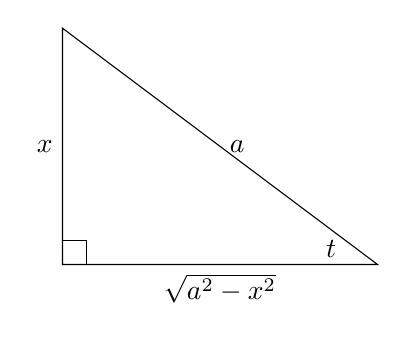
\begin{tikzpicture}
							% 绘制直角三角形
							\draw (0,0) -- (4,0) -- (0,3) -- cycle;
							% 标记直角符号
							\draw (0.3,0) -- (0.3,0.3) -- (0,0.3);
							% 标记角度
							\draw (3.6,0.2) arc (2:atan(3/4):0) node[midway,left] {$t$};
							% 标记边长
							\draw (2,0) node[below] {$\sqrt{a^2-x^2}$};
							\draw (0,1.5) node[left] {$x$};
							\draw (2,1.5) node[right] {$a$};
						\end{tikzpicture}
					\end{figure}
				\end{column}
			\end{columns}
			\pause
			\vspace{0.1cm}
			因此,
			$$
				\int a\cos t\cdot a\cos t\mathrm{~d}t = a^2\int \frac{\cos 2t+1}{2}\mathrm{~d}t=\frac{a^2}{2}\sin t\cos t+\frac{a^2}{2}t+C.
			$$
			\qed
		\end{exampleblock}
	}
\end{frame}

\begin{frame}
	\frametitle{变量代换法}
	\everymath{\displaystyle}
	{\small
		\begin{exampleblock}{$\color{black}\int \frac{\mathrm{~d} x}{\sqrt{x^2+a^2}}=\ln \left(x+\sqrt{x^2+a^2}\right)+C \quad(a>0)$}
			\begin{columns}
				\begin{column}{0.4\textwidth}
					% 左边的输入
					\pause 考虑合适的变换, 令
					$$
						x=a \tan t,\,\,t=\arctan\frac{x}{a}.
					$$
					\pause 于是有
					$$
						\sqrt{a^2+x^2} = a\sec t,\,\,\mathrm{~d} x=a \sec ^2 t \mathrm{~d} t.
					$$
					\pause 因此,
					$$
						\int \frac{\mathrm{~d} x}{\sqrt{x^2+a^2}}=\int \sec t \mathrm{~d} t.
					$$
				\end{column}
				\pause
				\begin{column}{0.5\textwidth}
					% 右边的图片
					\begin{figure}
						\centering
						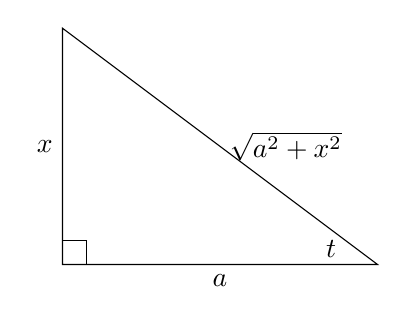
\begin{tikzpicture}
							% 绘制直角三角形
							\draw (0,0) -- (4,0) -- (0,3) -- cycle;
							% 标记直角符号
							\draw (0.3,0) -- (0.3,0.3) -- (0,0.3);
							% 标记角度
							\draw (3.6,0.2) arc (2:atan(3/4):0) node[midway,left] {$t$};
							% 标记边长
							\draw (2,0) node[below] {$a$};
							\draw (0,1.5) node[left] {$x$};
							\draw (2,1.5) node[right] {$\sqrt{a^2+x^2}$};
						\end{tikzpicture}
					\end{figure}
				\end{column}
			\end{columns}
			\vspace{0.1cm}
			\pause
			因此,
			$$
				\int \sec t \mathrm{~d} t= \ln |\sec t+\tan t|+C=\ln \left(x+\sqrt{x^2+a^2}\right)+C
			$$
			\qed
		\end{exampleblock}
	}
\end{frame}

\begin{frame}
	\frametitle{变量代换法}
	\everymath{\displaystyle}
	{\small
		\begin{exampleblock}{$\color{black}\int \frac{x^3}{\left(x^2-2 x+2\right)^2} \mathrm{~d} x=\frac{1}{2} \ln \left(x^2-2 x+2\right)+2 \arctan (x-1)-\frac{x}{x^2-2 x+2}+C$}
			\pause 考虑合适的变换, 令
			$$
				x^2-2 x+2=\sec ^2 t,\,\,x-1=\tan t .
			$$
			\pause 于是有
			$$
				\int \frac{x^3}{\left(x^2-2 x+2\right)^2} \mathrm{~d} x=\int \frac{(\tan t+1)^3}{\sec ^4 t} \cdot \sec ^2 t \mathrm{~d} t.
			$$
			\pause 因此,
			$$
				\begin{aligned}
					\int \frac{(\tan t+1)^3}{\sec ^4 t} \cdot \sec ^2 t \mathrm{~d} t & =\int\left(\sin ^3 t \cos ^{-1} t+3 \sin ^2 t+3 \sin t \cos t+\cos ^2 t\right) \mathrm{d} t \\
					\pause                                                            & =\int\left(\sin ^2 t \cos ^{-1} t+3 \cos t\right) \sin t \mathrm{~d} t                      \\
					\pause                                                            & \quad +\int\left(3 \sin ^2 t+\cos ^2 t\right) \mathrm{d} t
				\end{aligned}
			$$
		\end{exampleblock}
	}
\end{frame}

\begin{frame}
	\frametitle{}
	\everymath{\displaystyle}
	\begin{exampleblock}{}
		$$
			\begin{aligned}
				 & \pause =\int\left[\left(1-\cos ^2 t\right) \cos ^{-1} t+3 \cos t\right][-\mathrm{d}(\cos t)]+\int(2-\cos 2 t) \mathrm{d} t \\
				 & \pause =-\int\left(\cos ^{-1} t+2 \cos t\right) \mathrm{d}(\cos t)+2 t-\frac{1}{2} \sin 2 t                                \\
				 & \pause =-\ln \cos t-\cos ^2 t+2 t-\sin t \cos t+C
			\end{aligned}
		$$
		\pause 回忆辅助三角形, 有
		\begin{figure}
			\centering
			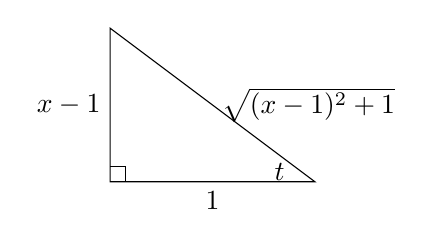
\begin{tikzpicture}[scale=0.65]
				% 绘制直角三角形
				\draw (0,0) -- (4,0) -- (0,3) -- cycle;
				% 标记直角符号
				\draw (0.3,0) -- (0.3,0.3) -- (0,0.3);
				% 标记角度
				\draw (3.6,0.2) arc (2:atan(3/4):0) node[midway,left] {$t$};
				% 标记边长
				\draw (2,0) node[below] {$1$};
				\draw (0,1.5) node[left] {$x-1$};
				\draw (2,1.5) node[right] {$\sqrt{(x-1)^2+1}$};
			\end{tikzpicture}
		\end{figure}
		\pause 因此
		$$
			\cos t=\frac{1}{\sqrt{x^2-2 x+2}}, \sin t=\frac{x-1}{\sqrt{x^2-2 x+2}},
		$$
		\pause
		{\small $\color{black}\int \frac{x^3}{\left(x^2-2 x+2\right)^2} \mathrm{~d} x=\frac{1}{2} \ln \left(x^2-2 x+2\right)+2 \arctan (x-1)-\frac{x}{x^2-2 x+2}+C.$}

		\qed
	\end{exampleblock}
\end{frame}

\begin{frame}
	\frametitle{练习题}
	\everymath{\displaystyle}
	\begin{exampleblock}{$\color{black}\int \frac{1}{x+\sqrt{1-x^2}} \mathrm{~d} x=\frac{1}{2} \arcsin (x)+\frac{1}{2} \ln \left|x+\sqrt{1-x^2}\right|+C$}
		令
		$
			\sin t =x,\,\,\mathrm{~d}x=\cos t\mathrm{d}t,
		$
		那么
		$$
			\int \frac{1}{x+\sqrt{1-x^2}} \mathrm{~d} x=\int \frac{\cos t}{\sin t+\cos t}\mathrm{~d}t.
		$$\\
		因此
		\begin{align*}
			\int \frac{\cos t}{\sin t+\cos t}\mathrm{~d}t & =\int \frac{\frac{1}{2}(\cos t + \sin t)+ \frac{1}{2}(\cos t - \sin t)}{\sin t+\cos t}\mathrm{~d}t \\
			                                              & =\int \frac{1}{2}\mathrm{~d}t+ \frac{1}{2}\int \frac{\mathrm{d}(\sin t+\cos t)}{\sin t+\cos t}     \\
			                                              & =\frac{1}{2}t+\frac{1}{2}\ln\left|\sin t + \cos t\right|+C.
		\end{align*}
	\end{exampleblock}
\end{frame}

\begin{frame}
	\frametitle{练习题}

	\begin{exampleblock}{}
		建立辅助三角形:
		\begin{figure}
			\centering
			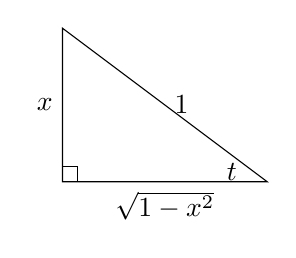
\begin{tikzpicture}[scale=0.65]
				% 绘制直角三角形
				\draw (0,0) -- (4,0) -- (0,3) -- cycle;
				% 标记直角符号
				\draw (0.3,0) -- (0.3,0.3) -- (0,0.3);
				% 标记角度
				\draw (3.6,0.2) arc (2:atan(3/4):0) node[midway,left] {$t$};
				% 标记边长
				\draw (2,0) node[below] {$\sqrt{1-x^2}$};
				\draw (0,1.5) node[left] {$x$};
				\draw (2,1.5) node[right] {$1$};
			\end{tikzpicture}
		\end{figure}
		可以得到:
		$$
			t=\arcsin x,\,\,\sin t = x,\,\,\cos t = \sqrt{1-x^2}.
		$$
		因此, 可以得到
		$$
			\begin{aligned}
				\int \frac{1}{x+\sqrt{1-x^2}} \mathrm{~d} x & = \frac{1}{2}t+\frac{1}{2}\ln\left|\sin t + \cos t\right|+C                 \\
				                                            & =\frac{1}{2} \arcsin (x)+\frac{1}{2} \ln \left|x+\sqrt{1-x^2}\right|+C.\qed
			\end{aligned}
		$$
	\end{exampleblock}
\end{frame}

\begin{frame}
	\frametitle{练习题}
	\everymath{\displaystyle}
	{\small
		\begin{exampleblock}{$\color{black}\int \frac{\mathrm{d} x}{x \sqrt{x^2-1}}$}
			建立辅助三角形:
			\begin{figure}
				\centering
				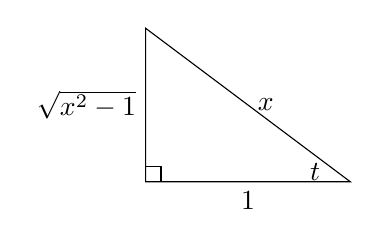
\begin{tikzpicture}[scale=0.65]
					% 绘制直角三角形
					\draw (0,0) -- (4,0) -- (0,3) -- cycle;
					% 标记直角符号
					\draw (0.3,0) -- (0.3,0.3) -- (0,0.3);
					% 标记角度
					\draw (3.6,0.2) arc (2:atan(3/4):0) node[midway,left] {$t$};
					% 标记边长
					\draw (2,0) node[below] {$1$};
					\draw (0,1.5) node[left] {$\sqrt{x^2-1}$};
					\draw (2,1.5) node[right] {$x$};
				\end{tikzpicture}
			\end{figure}
			建立变换
			$$
				\frac{1}{x}=\sec t,\,\,\frac{1}{\sqrt{x^2-1}}=\cot t,\,\,\mathrm{~d}x=\tan t\sec t \mathrm{~d}t.
			$$
			因此,\\
			$$
				\int \frac{\mathrm{d} x}{x \sqrt{x^2-1}}=\int \cos t\cot t\cdot \sec t\tan t\mathrm{d}t=t+C=\arctan (\sqrt{x^2-1})+C.
			$$
		\end{exampleblock}
	}
\end{frame}

\begin{frame}
	\frametitle{练习题}
	\everymath{\displaystyle}
		\begin{exampleblock}{$\color{black}\int x(2 x-1)^{100} \mathrm{~d} x=\frac{(2 x-1)^{101}}{4}\left(\frac{2 x-1}{102}+\frac{1}{101}\right)+C$}
			令 $2 x-1=t$ 即 $x=\frac{t+1}{2}$, 则 $\mathrm{d} x=\frac{1}{2} \mathrm{~d} t$, 于是
			$$
				\begin{aligned}
					\int x(2 x-1)^{100} \mathrm{~d} x & =\frac{1}{4} \int(t+1) t^{100} \mathrm{~d} t=\frac{1}{4}\left(\frac{t^{102}}{102}+\frac{t^{101}}{101}\right)+C \\
					                                  & =\frac{(2 x-1)^{101}}{4}\left(\frac{2 x-1}{102}+\frac{1}{101}\right)+C
				\end{aligned}
			$$
		\end{exampleblock}
\end{frame}

\begin{frame}
	\frametitle{练习题}
	\everymath{\displaystyle}
	\begin{block}{}
		\begin{columns}[onlytextwidth]
			\begin{column}{0.5\textwidth}
				\begin{enumerate}
					\item $\int x^2(x+1)^n \mathrm{~d} x$
					\item $\int \frac{\mathrm{d} x}{x \sqrt{1+x^2}}$
				\end{enumerate}
			\end{column}
			\begin{column}{0.5\textwidth}
				\begin{enumerate}
					\setcounter{enumi}{2}
					\item $\int \frac{\ln x \mathrm{~d} x}{x \sqrt{1+\ln x}}$
					\item $\int \frac{\sin ^2 x}{\cos ^6 x} \mathrm{~d} x$
				\end{enumerate}
			\end{column}
		\end{columns}
	\end{block}
	\begin{exampleblock}{}
				\begin{enumerate}
					\pause \item $\left(\frac{1}{n+1}-\frac{2(x+1)}{n+2}+\frac{(x+1)^2}{n+3}\right)(x+1)^{n+1}+C$;
					\pause \item $\ln\left|\frac{\sqrt{1+x^2}-1}{x}\right|+C$;
					\pause \item $\frac{2}{3}(\ln x-2) \sqrt{1+\ln x}+C$;
					\pause \item $\frac{1}{5} \tan ^5 x+\frac{1}{3} \tan ^3 x+C$,
				\end{enumerate}
	\end{exampleblock}
\end{frame}

\section{分部积分}

\begin{frame}
	\frametitle{从微分计算法则到不定积分计算法则}
	回顾不定积分的乘积运算法则:\pause
	\begin{block}{}
		\begin{enumerate}
			\item 乘积法则:
			      \begin{itemize}
				      \item \pause 微分的乘积法则:
				            $$
					            u\mathrm{~d}v+v\mathrm{~d}u =\mathrm{~d}(uv).
				            $$
				      \item \pause 不定积分的乘积法则:
				            $$
					            \int u\mathrm{~d}v+\int v\mathrm{~d}u=\int\mathrm{~d}(uv) = uv.
				            $$
				            \pause 最后这一条经常被称为分部积分公式.
			      \end{itemize}
		\end{enumerate}
	\end{block}
\end{frame}

% Thank you page
\beamertemplateshadingbackground{structure.fg!90}{structure.fg}
\begin{frame}[plain]
	\vfill
	\centering
	{
		\centering \Huge \color{white} Thank you for your attention!\\[10pt]Questions?
	}
	\vfill
\end{frame}


\end{document}


